\chapter{Methodology}
\label{sec:methodology}

This chapter outlines the research method designed to create and assess a multimodal Automatic Personality Recognition (APR) framework for Filipino Instagram users. This framework will tackle the specific language and cultural challenges found in the dataset, including code switching and unique patterns of visual self-expression. The process starts with  preprocessing, followed by exploratory data analysis and feature extraction from text, images, and metadata. It also includes an early combination of these features. Finally, we will train machine learning models and thoroughly evaluate them to see how well they perform in predicting users' personality traits.

\begin{figure}[H]
	\centering
	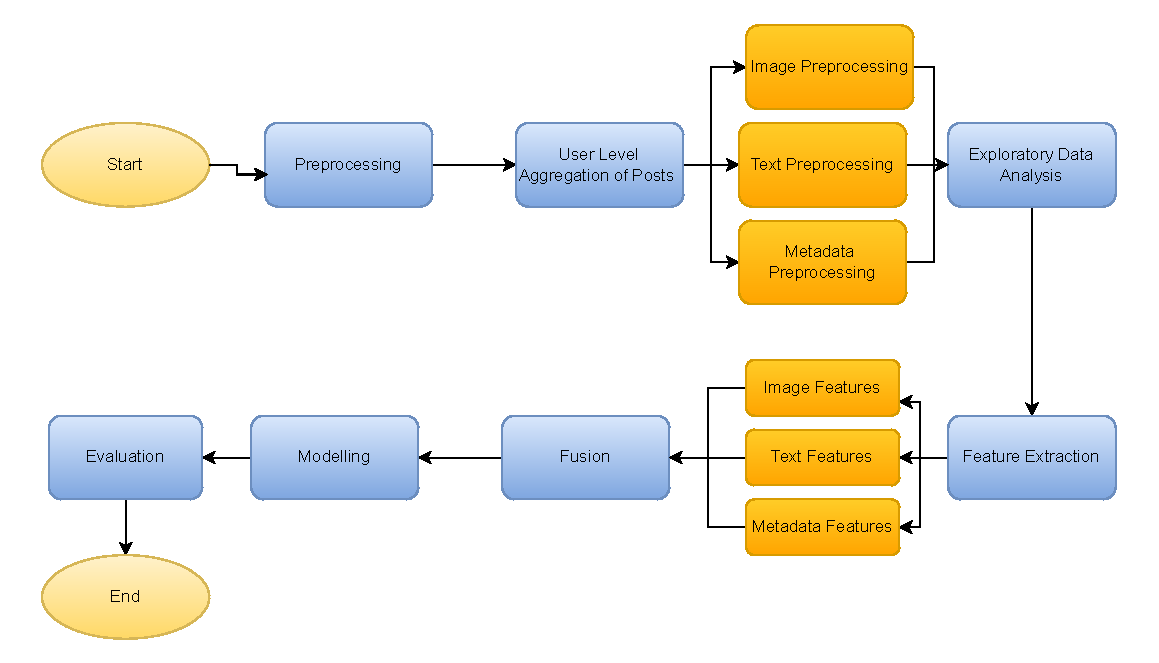
\includegraphics[width=\textwidth]{"figures/Methodology-Flowchart.pdf"}
	\caption{Methodology Flowchart}
	\label{fig:methodology_pipeline}
\end{figure}

\section{Data Source}
\label{sec:data}
This research is grounded in the Instagram subset of the PagkataoKo dataset, a comprehensive resource specifically curated for Filipino APR studies \citep{tighe_acorda_2022}. The dataset's inclusion of user-generated content (posts and images), demographic information, and self-reported Big Five personality scores makes it an ideal foundation for this supervised machine learning investigation. The original Instagram subset contains data from 1,380 participants who provided access to their accounts, totaling 195,757 posts.

\subsection{Data Collection Methodology}
The data was gathered between the first week of June 2019 and the second week of February 2020 through a purpose-built web application. This tool streamlined the collection process by first presenting participants with a consent form and study directions. Upon granting consent, participants chose whether to authorize the application to access their social media data from Instagram only, Twitter only, or both. Following this automated collection, participants completed a demographic questionnaire and the 44-item Big Five Inventory (BFI-44) to assess their personality traits.

The application used the official Instagram Legacy API and Twitter API v1. For Instagram, the application collected post data (captions and image links) of as many posts as the API would return, a link to the profile picture, and account metadata. Only links to images were collected to reduce strain on the application. If a post contained multiple photos, only the link to the first photo was collected. Posts that contained videos were discarded. Due to the observed behavior of image URLs changing over time, the images of collected links were downloaded at the end of each day of collection to avoid losing access \citep{tighe_acorda_2022}. 

\subsection{Participant Sampling and Filtering}
A mixed sampling strategy was employed to recruit participants. The initial phase utilized convenience and snowball sampling, where information about the study was disseminated within the researchers' immediate networks. To reach a broader Filipino audience, this was followed by a series of targeted online advertisement campaigns on Facebook, Instagram, and Twitter.

From an initial pool of 3,186 participants, a filtering process was applied to ensure relevance to the Filipino context. Only individuals who identified their nationality as either "Filipino" or "mixed-Filipino" were retained, resulting in a final cohort of 3,128 individuals whose data comprises the full PagkataoKo dataset \citep{tighe_acorda_2022}.


\subsection{Data Characteristics}
This study is only concerned with the Instagram portion of the dataset, which comprises 44.1\% of the data or 1,380 respondents who authorized access to their accounts. The posts collected were made over a 10-year period prior to the data collection (2010-2020) \citep{tighe_acorda_2022}. Detailed numerical characteristics of this subset can be seen in Table~\ref{tab:pagkataoko_data_characteristics}. Further details such as participant demographics and language use are discussed in Section~\ref{subsec:eda}.

\begin{table}[h!]
\centering
\caption{Data characteristics of user-generated and account-related data across the Instagram subset of the PagkataoKo dataset}
\label{tab:pagkataoko_data_characteristics}
\begin{tabular}{@{}llr@{}}
\toprule
\textbf{Data} & \textbf{Statistics} & \textbf{Count} \\ 
\midrule
    {Collected Posts} & Total & 195,757 \\
    & Average & 141.85 \\
    & SD & 224.00 \\
    & Min / Max & 0 / 1,902 \\
    & \# w/ Caption & 178,650 \\
    & \# w/ Image & 162,500 \\
\midrule
    {Acct. Recorded Posts} & Average & 146.60 \\
    & SD & 267.99 \\
    & Min / Max & 0 / 5,680 \\
\midrule
    {Following Count} & Average & 470.39 \\
    & SD & 442.85 \\
    & Min / Max & 0 / 6,338 \\
\midrule
Profile Pictures & Total & 1,030 \\
\bottomrule
\end{tabular}
\begin{minipage}{\linewidth}
\small\textit{Note.} Adapted from \textit{Data characteristics of user-generated and account-related data across three participant subsets (Table 3)} \citep{tighe_acorda_2022}.
\end{minipage}
\end{table}


\subsection{Personality Score Transformation to Labels}
In its raw form, the PagkataoKo dataset provides personality scores as continuous numerical values ranging from 1.0 to 5.0 for each of the Big Five traits. Since this study frames personality recognition as a classification task, these continuous scores must be transformed into discrete labels.

To achieve this, a \textbf{median split} will be performed for each of the five personality traits independently. This choice is informed by the findings of Aviles et al. (2023), who explored eight different discretization methods on Filipino social media data. Their study found that while methods that remove a large number of participants (such as LHNASD, which removed 70\% of the data) can achieve the highest performance, the LH Median method provided the best balance between performance and data retention. Specifically, the LH Median method achieved the second-highest average Kappa score while only removing a small fraction of participants (approximately 6\%) whose scores fell exactly on the median \citep{aviles2023}. Given this trade-off, the median split is selected as a robust and practical approach that preserves the vast majority of the dataset while still creating distinct high and low classes for the models.

For a given trait (e.g., Openness), users with a score above the median value for that trait will be assigned the 'High' label (e.g., 'High-Openness'). Users with scores at or below the median will be assigned the 'Low' label (e.g., 'Low-Openness'). This process will result in five separate binary labeling schemes, one for each personality dimension, which will serve as the target variables for the classification models.

\begin{figure}[H]
	\centering
	% Placeholder for the actual diagram image
	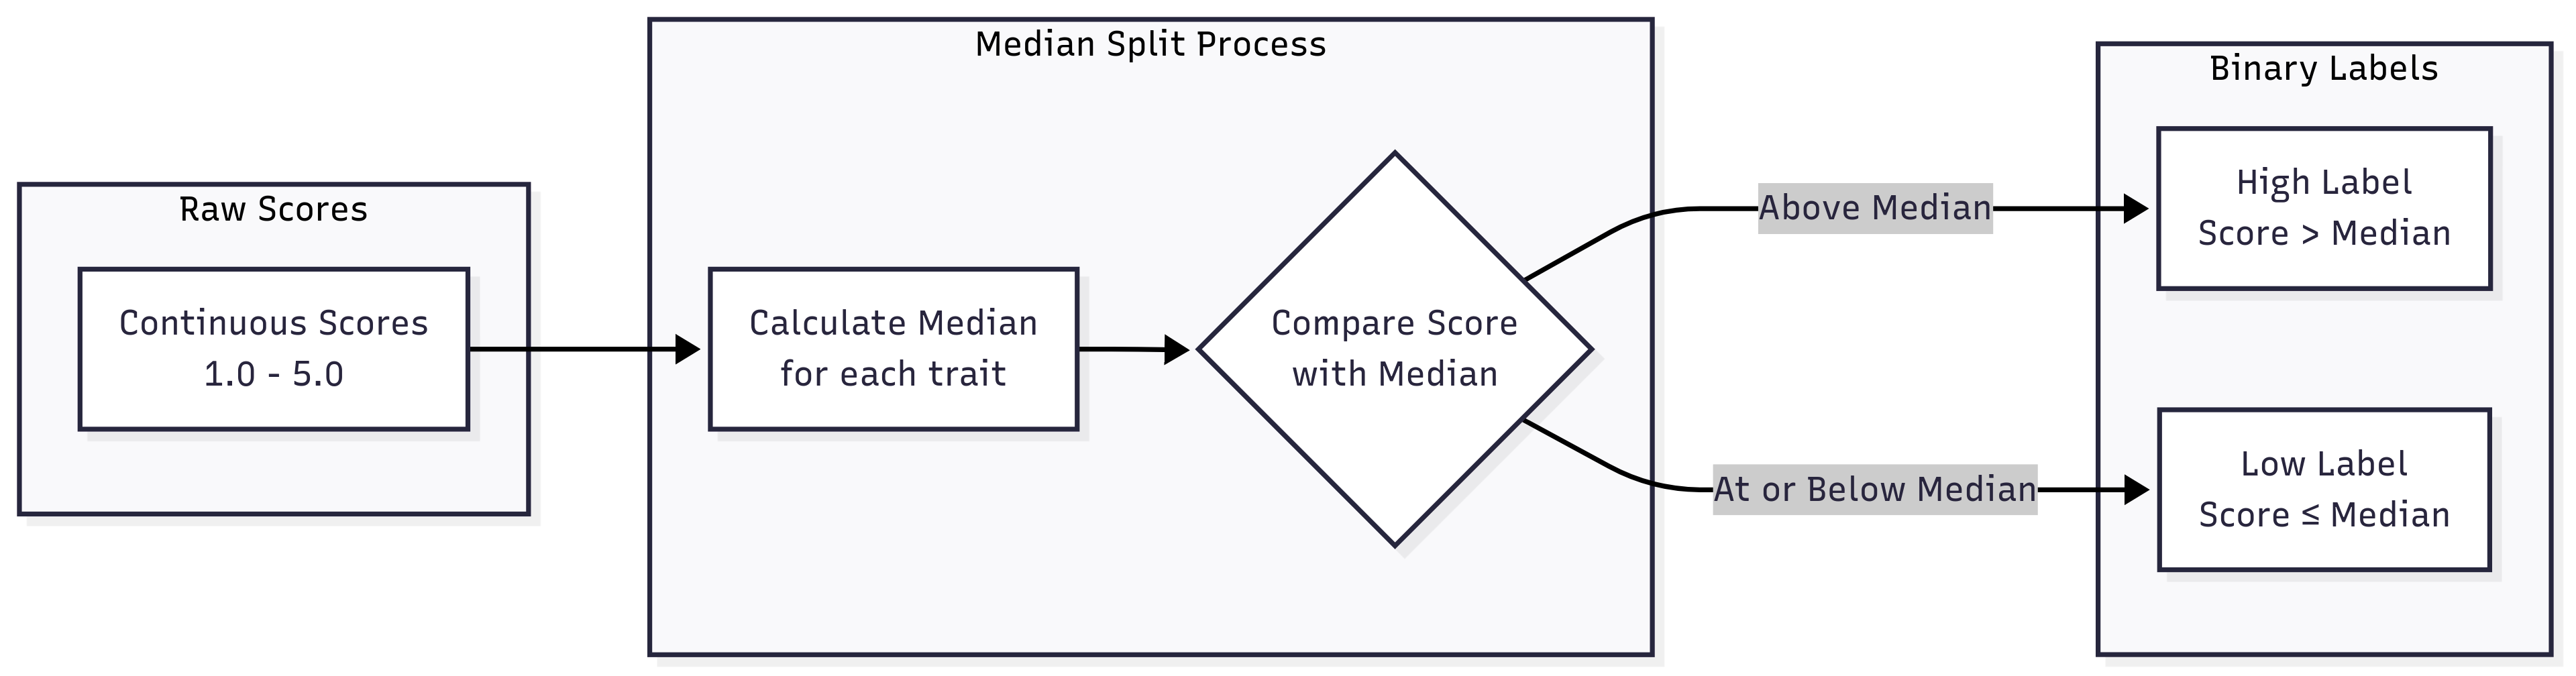
\includegraphics[width=1\textwidth]{"figures/Scores.png"}
	\caption{Category to Label via Median Split}
	\label{fig:median_split_diagram}
\end{figure}


\subsection{Data Splitting}
For model training and evaluation, the dataset will be divided using a user-level stratified split for model training and evaluation: \textbf{70\%} for training, \textbf{15\%}for validation, and \textbf{15\%} for testing. To ensure that the proportion of 'High' and 'Low' labels for each personality trait is consistent across these sets, the split will be stratified based on the generated personality labels. This helps prevent model bias and ensures that the models are trained and evaluated on representative distributions of each personality class.

\section{Preprocessing}
This stage cleans and organizes the raw data to make it suitable for feature extraction. The main task is \textbf{user-level aggregation}. Here, all posts, images, and metadata for a single user are collected into a single behavioral profile. 

\subsection{Image Preprocessing}
All images will go through preprocessing to get them ready for the \textbf{ResNet50} model. Each image will be resized to 224x224 pixels to fit the model’s required input size. We will also check for corrupted image files. Any posts with unreadable images will be flagged and excluded from the image-based feature extraction process.

\subsection{Text Preprocessing}
A basic text cleaning method will be used to keep as much of the original content as possible, including multilingual text. The process will involve breaking down the raw caption text into tokens and replacing things like URLs and user mentions with generic tokens (e.g., URL, USER) instead of removing them completely. This way, we keep the context of where a link or mention appeared. All languages will be kept in the text.


\section{Exploratory Data Analysis}
\label{subsec:eda}

Before feature extraction, we will conduct exploratory data analysis (EDA) to understand the key features of the dataset. This analysis will aim to pinpoint demographic trends and content patterns that can guide feature engineering and model interpretation.

The demographic distribution of the final 1,300-user subset, as derived from the PagkataoKo dataset paper, is summarized in Table 4.1. The data shows a user base that is predominantly young (49.3\% aged 18-20) and female (78.0\%).

As detailed by \citet{tighe_acorda_2022}, the language of each post was determined using a majority vote between two language identifiers (Polyglot and FastText).Posts where the identifiers agreed were labeled as either 'English' (75.6\%) or 'Tagalog' (4.3\%). Posts where the identifiers did not agree were assigned a 'Conflict' label (19.4\%), a category understood to primarily represent posts containing code-switching or other forms of mixed-language use.

\begin{table}[h]
	\centering
	\caption{Demographic distribution of Instagram subset (n=1,300)}
	\label{tab:demo}
	\begin{tabular}{lcc}
		\hline
		\textbf{Characteristic} & \textbf{Category} & \textbf{Percentage} \\ \hline
		\textbf{Age} & 18-20 & 49.3\% \\
		& 21-23 & 31.3\% \\
		& 24-26 & 10.7\% \\
		& $\geq$27 & 8.8\% \\ \hline
		\textbf{Sex} & Female & 78.0\% \\
		& Male & 20.0\% \\
		& Intersex/ Declined & 2.0\% \\ \hline
		\textbf{Language} & English & 75.6\% \\
		& Tagalog & 4.3\% \\
		& Code-switched & 19.4\% \\ \hline
	\end{tabular}
\end{table}
% --- REVISION G START: Added new section for PCA Rationale ---
\section{Feature Engineering}
\label{subsec:features}
This stage converts the raw, multimodal data associated with each Instagram user—comprising images, textual captions, and account metadata—into a single, quantitative feature vector. This vector is designed to be processed by supervised machine learning algorithms (logistic regression, support vector machines, and XGBoost) for the task of personality trait prediction. Our study primarily employs \textbf{average pooling}, which involves computing the mean of all feature vectors for a given user. This aggregation strategy is deliberately chosen to align with the theoretical view of personality as a stable, long-term construct \citep{babcock2020big}. By averaging a user's content features over many posts, the resulting vector represents their typical behavior and expressive style, effectively smoothing out outlier content that may not be representative of their core personality \citep{azucar_predicting_2018}. This approach aims to capture the consistent 'trait' aspect of a user, rather than a transient emotional 'state' that might be reflected in a single post.


The process is divided into three parallel pipelines, one for each data modality.

\subsection{Image Modality Pipeline}
This pipeline processes all valid images from a user's profile to extract a comprehensive set of visual features. For each image, the following features are extracted in parallel before being aggregated to the user level.

\subsubsection{High-Level Semantic Features via ResNet50}
The pre-trained \textbf{ResNet50} convolutional neural network is used as a feature extractor. For each image, a \textbf{2,048-dimension feature vector} is extracted from the output of the final average pooling layer. This vector captures abstract visual concepts, objects, and textures.

ResNet50 was chosen because it demonstrates higher classification accuracy on benchmark datasets like ImageNet, is substantially more efficient in terms of model size (98 MB vs. 549 MB for VGG19), and its residual connections allow for the effective training of deeper networks, enabling the model to learn more complex feature representations without suffering from the vanishing gradient problem that can affect older architectures \citep{he2015, simonyan2014very}.

\subsubsection{Object and Scene Recognition via the Imagga API}
To quantify the semantic content and social context of the images, this study leverages the \textbf{Imagga API}, a commercial computer vision service.

Imagga is a cloud-based service that provides a suite of powerful image analysis tools through a simple API. Its core functions include automated image tagging, categorization, color extraction, and content moderation, all powered by pre-trained deep learning models capable of recognizing thousands of objects, scenes, and concepts \citep{imagga_website, imagga_solutions}. The Imagga API was selected for its robust, recognition capabilities, which provide a reliable method for extracting semantic features without the significant overhead of training a custom object detection model. Its structured JSON output is easily parsed and integrated into the feature engineering pipeline, making it a pragmatic and efficient choice for this research \citep{imagga_docs}.

While the Imagga API's general model is capable of recognizing over 3,000 distinct objects and concepts \citep{imagga_solutions}, creating a feature vector of this size for each user would be computationally inefficient and result in a highly sparse feature space. To create a more dense and manageable feature set, a fixed-size vocabulary of the most relevant tags will be established. This is a standard approach analogous to a bag-of-words model in text processing \citep{salton1975}. A vocabulary of the top N=200 most frequent tags across the entire dataset will be identified. Subsequently, for each user, a \textbf{200-dimension feature vector} will be constructed, where each dimension represents the frequency of one of these top tags appearing in that user's posts.

Our study specifically utilizes the \texttt{/tags} endpoint of the Imagga API. For each image submitted, the API returns a JSON object containing a list of detected tags (e.g., "person," "selfie," "food," "beach") and a corresponding confidence score (from 0 to 100) for each tag \citep{imagga_docs}. These tags are used to construct features such as the frequency of posts containing people, selfies, or specific objects, which have been linked in prior literature to traits like Extraversion.

\begin{figure}[H]
	\centering
	\begin{verbatim}
		{
			"result": {
				"tags": [
				{ "confidence": 95.4, "tag": { "en": "beach" } },
				{ "confidence": 88.1, "tag": { "en": "ocean" } },
				{ "confidence": 75.9, "tag": { "en": "person" } },
				{ "confidence": 62.3, "tag": { "en": "sunset" } }
				]
			}
		}
	\end{verbatim}
	\caption{ \texttt{Sample JSON Output from the Imagga API /tags Endpoint. An illustrative, non-dataset-specific example of the JSON response for an image of a person at a beach during sunset.}}
	\label{fig:imagga_json}
\end{figure}

Furthermore, the use of Imagga is also for feasibility due to the Imagga JSON tags already being a part of the PagkataoKo Dataset.
\subsubsection{Low-Level Photo Characteristics Analysis}
To capture the aesthetic qualities of images, a set of low-level features is extracted.

For each image, color features are derived using the HSV (Hue, Saturation, Value) color space. The inclusion of these features is based on the works of \citet{ferwerda2016} and \citet{Ferwerda2018}, whose studies are very similar to ours in that they conducted APR using Instagram photos and were able to find some correlations between some of these features and Big Five personality traits. These features are also found in the work of \citet{Branz2020}, who also tackled Instagram photo-based APR. 

\begin{itemize} \item \textbf{Hue-related Features:} The range of the Hue (H) parameter is divided into six intervals corresponding to the primary hues: red, orange, yellow, green, blue, and violet. For each hue, the share of the image surface it covers is calculated by dividing the number of pixels in that hue's interval by the total number of pixels. Furthermore, these are merged into composite features representing the share of \textit{warm colors} (red, orange, yellow) and \textit{cold colors} (green, blue, violet). \item \textbf{Saturation-related Features:} For each image, the mean saturation and saturation variance are calculated. The saturation axis is also divided into three equally spaced intervals (low, mid, high), and the share of pixels falling into each interval is computed. These features quantify whether an image's colors are bleak and colorless (low saturation), vivid (high saturation), or a mix of both (high variance). \item \textbf{Value-related Features:} The mean and variance of the Value (V) parameter are calculated across all pixels to represent how light or dark an image is and its level of contrast, respectively. Similar to saturation, the value axis is divided into three intervals (low, mid, high), and the share of pixels in each is calculated to quantify the presence of dark and light areas. \item \textbf{Pleasure-Arousal-Dominance (PAD) Features:} To model the emotional expression conveyed by an image's color properties, the PAD model by \citet{Valdez1994} is adopted. This model computes three composite features as a linear combination of the average Value (V) and Saturation (S) levels: \begin{itemize} \item Pleasure = $0.69 \times V + 0.22 \times S$ \item Arousal = $-0.31 \times V + 0.60 \times S$ \item Dominance = $-0.76 \times V + 0.32 \times S$ \end{itemize} \end{itemize} 

All of these post-level aesthetic features are then aggregated to the user level by calculating their average values across all of a user's images, creating a comprehensive aesthetic profile.


\subsection{Text Modality Pipeline}
This pipeline processes all textual captions from a user's posts to extract linguistic and semantic features.

\subsubsection{Contextual Embeddings from TF-IDF}
To capture deep contextual meaning from the user's captions, this study will utilize \textbf{TF-IDF} model will be used to generate embeddings for the text. Its training corpus includes the text captions of 178,650 Instagram posts collected in the Pagkatao dataset \citep{tighe_acorda_2022}. For each user's aggregated captions, the TF-IDF model will produce a sparse feature vector. The dimensionality of this vector will be equal to the vocabulary size of the training corpus. Based on the full PagkataoKo Instagram subset, which contains 92,030 unique tokens, the final dimension will be a substantial subset of this size.




\begin{comment}
While traditional methods like TF-IDF capture lexical importance, they fail to understand context, semantics, or word order. BERT (Bidirectional Encoder Representations from Transformers) models do well in natural language understanding and have been shown to significantly outperform TF-IDF in personality classification tasks. For example, a study by \citet{zhang2023} directly comparing the two approaches for MBTI personality prediction found that a fine-tuned BERT model paired with a Logistic Regression classifier achieved an average accuracy of 87.7\%, a notable improvement over the 84.3\% accuracy achieved by the same classifier using a traditional TF-IDF vectorizer \citep{zhang2023}. BERT's key advantage is its ability to generate contextual embeddings; the representation of a word changes based on the words surrounding it. Given the dataset's mix of English, Tagalog, and code-switching, a multilingual BERT model is particularly suitable, as it has been pre-trained on a corpus of over 100 languages and can effectively handle the linguistic complexity of the data \citep{devlin2018bert, cruz2022roberta}.
\end{comment}

\subsubsection{Word Embedding Representation}
As a complementary feature to the contextual embeddings from TF-IDF, pre-trained \textbf{Word2Vec} word embeddings will also be used to capture a static, non-contextual representation of semantic meaning \citep{Mikolov_Sutskever_Chen_Corrado_Dean_2013}. For each user, the embeddings for all words in their captions will be combined by computing the mean of the vectors (average pooling). This results in a single, dense vector for each user that represents the aggregate meaning of their posts.


The pre-trained model to be used is from \citet{velasco2021filwembs} that contains “texts from Tagalog Wikipedia, news articles, and tweets.” Its data source comes from \citet{Cruz_Cheng_2019}’s \textit{WikiText-TL-39}, \citet{Cruz_Resabal_Lin_Velasco_Cheng_2021}’s \textit{NewsPH-NLI}, and an unpublished Twitter dataset. Preprocessing techniques, such as “removing quotes and its contents” \citet{velasco2021filwembs}, are done before proceeding to perform word embedding.


\subsection{Metadata Modality Pipeline}
Behavioral signals are extracted from user account metadata. As noted in the PagkataoKo dataset paper, the Instagram subset provides two key account-level metrics: the total number of posts a user has made (\texttt{PostCount}) and the number of other accounts they follow (\texttt{FollowingCount}) \citep{tighe_acorda_2022}.

This pipeline involves two key steps:
\begin{enumerate}
	\item \textbf{Feature Extraction:} The raw numerical values for \texttt{PostCount} and \texttt{FollowingCount} are extracted for each user.
	\item \textbf{Normalization:} These features exist on vastly different scales; for example, a user might have 100 posts but follow 1,000 accounts. To prevent algorithms that are sensitive to feature magnitude (such as Support Vector Machines) from giving undue weight to features with larger numerical ranges, all metadata features are scaled to a fixed range of  using min-max normalization.
\end{enumerate}
This preprocessing step is for ensuring that the metadata features contribute fairly to the final model alongside the features from the image and text modalities. The final output of this pipeline is a 2-dimensional, normalized metadata feature vector for each user.

\subsection{Dimensionality Reduction as an Optional Step}
The primary methodological approach of this study is to utilize the full, high-dimensional feature vectors generated from the ResNet50 (2,048 dimensions) and TF-IDF (vocabulary size). This decision is motivated by a core research objective: to maintain the highest possible level of interpretability. Applying dimensionality reduction techniques like PCA transforms the original features into a new set of components, which can make it difficult to trace a prediction back to the specific, original visual or textual cues (e.g., a particular object in an image or a specific word in a caption).

However, should initial modeling experiments with the full feature set yield poor performance, show significant signs of overfitting, or prove to be computationally prohibitive, \textbf{Principal Component Analysis (PCA)} will be explored as an optional, secondary step. In this contingency, PCA would be applied to the aggregated ResNet50 and TF-IDF feature sets to create a more compact and less noisy representation before feature fusion. This two-stage approach allows the study to first prioritize interpretability while retaining a robust method for managing dimensionality if it proves necessary.

\subsection{Feature Pipelines}
These diagrams illustrate the flow of data from its raw form through the parallel feature engineering pipelines to the final aggregated user vector. 

The final value of $k$ for each feature set will be determined empirically during implementation. The table below represents an estimate for each the image feature pipeline and text feature pipeline.


\begin{figure}[H]
	\centering
	% Placeholder for the actual diagram image
	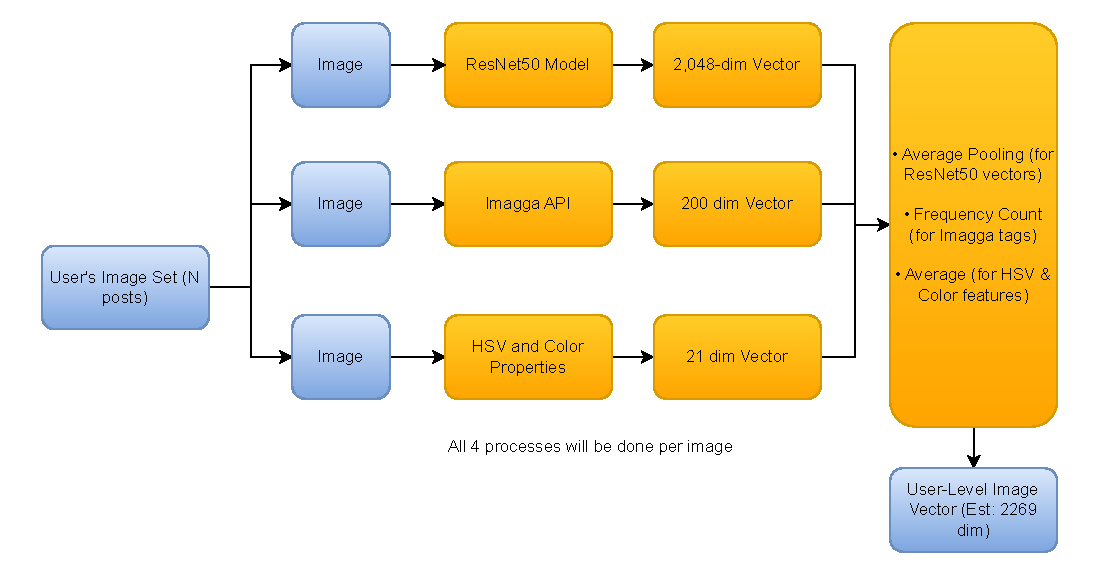
\includegraphics[width=\textwidth]{"figures/Image-Pipeline-Diagram.pdf"}
	\caption{The Image Feature Engineering Pipeline. }
	\label{fig:image_pipeline_diagram}
\end{figure}

Features are extracted from each image via three parallel processes: High-Level Semantics (ResNet50), Object Content (Imagga API), and Low-Level Aesthetics. These post-level features are then aggregated to the user level and concatenated. The final user-level image vector is a combination of these three feature sets, with an estimated total dimensionality of approximately 2,269 (2,048 from ResNet50 + \textasciitilde200 from top Imagga tags + 21 from aesthetic features).

\begin{figure}[H]
	\centering
	% Placeholder for the actual diagram image
	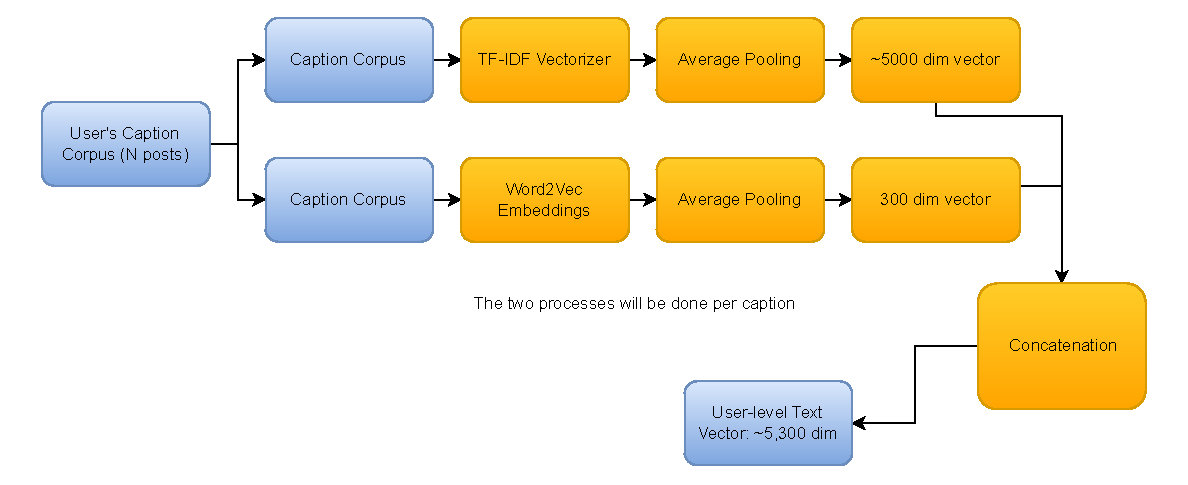
\includegraphics[width=\textwidth]{"figures/Text-Pipeline-Diagram.pdf"}
	\caption{The Text Feature Engineering Pipeline. }
	\label{fig:text_pipeline_diagram}
\end{figure}

A user's entire caption corpus is processed through two parallel paths to extract lexical features (TF-IDF) and semantic embeddings (Word2Vec). These are aggregated to the user level and concatenated. The final output is a user-level text vector. Its dimensionality will be the sum of the Word2Vec dimension (300) and the training set's vocabulary size (V) from TF-IDF, 


\begin{figure}[H]
	\centering
	% Placeholder for the actual diagram image
	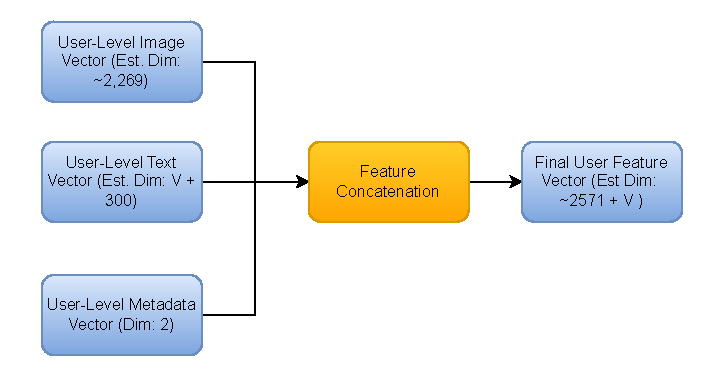
\includegraphics[width=\textwidth]{"figures/Fusion-Diagram.pdf"}
	\caption{User-Level Aggregation and Feature Fusion.}
	\label{fig:fusion_diagram}
\end{figure}

The outputs from the individual modality pipelines—the Image Vector (Est. Dim: \textasciitilde2,269), Text Vector (Est. Dim: \textasciitilde5,300), and Metadata Vector (Dim: 2)—are combined via feature concatenation. This process results in the final, unified user feature vector which serves as the input for the machine learning models.

\section{Feature Selection}
Following feature extraction, a feature selection step will be implemented to identify relevant predictors. The approach will vary based on the feature type.

For discrete, categorical features, such as the tags generated by the Imagga API, the \textbf{Chi-Squared ($\chi^2$) test of independence} will be used. This statistical method is well-suited for evaluating the association between each categorical feature and the binary 'High'/'Low' personality labels. Features that show a statistically significant association (indicated by a low p-value) will be considered highly relevant.

For the high-dimensional, dense features generated by ResNet50 and BERT, the Chi-Squared test is not appropriate. Instead, the relevance of these features will be assessed post-modeling using the interpretability techniques described in Section \ref{subsec:analysis}, such as SHAP. This allows for an evaluation of feature importance based on their actual contribution to the final model predictions.

\section{Early Feature Fusion}
\label{subsec:fusion}
This stage employs \textbf{early fusion} (also known as feature-level fusion) to combine the processed features from the image, text, and metadata pipelines into a single, unified representation for each user. The final user-level vectors from each of the three modality pipelines are concatenated to create a single, high-dimensional feature vector. This unified vector serves as the final input for the machine learning models.

\section{Model Training}
\label{subsec:models}

Three distinct classification models will be trained to predict the Big Five personality traits: Logistic Regression, a Support Vector Machine (SVM), and an XGBoost classifier. These models will be implemented using the \texttt{scikit-learn} \citep{pedregosa2011} and \texttt{XGBoost} \citep{chen2016} Python libraries.

A logistic regression (LR) model will be trained as a strong and interpretable baseline. Its performance will provide a benchmark to compare against the more complex models, making it easier to measure improvements.

A Support Vector Machine (SVM) will be trained, and its kernel function (e.g., Radial Basis Function (RBF), linear, polynomial) and regularization parameters \texttt{(C, gamma)} will be optimized through a comprehensive grid search to find the best setup for the data.

Lastly, we will also train an XGBoost classifier. This gradient-boosting algorithm effectively handles different types of features and includes a built-in way to assess the importance of those features.

\section{Model Analysis}
\label{subsec:analysis}
A detailed review will be done to assess how well the trained models perform. The main metrics for evaluation will be the \texttt{Macro-F1 score} and the \texttt{Area Under the Receiver Operating Characteristic Curve (AUC-ROC)}. We choose the Macro F1 score because it works well for datasets with uneven class distributions. The AUC-ROC will help us evaluate the model's ability to rank and differentiate between classes.

We will use \texttt{SHAP (SHapley Additive exPlanations)} to understand how the models make decisions. SHAP helps us measure how much each feature contributes to the model's predictions. This will create plots showing global feature importance, giving a clear ranking of the most impactful visual, textual, and metadata clues for each personality trait.

Lastly, a series of model analyses will be conducted. This involves training and evaluating separate models on distinct subsets of the full feature set. The same set of classifiers (Logistic Regression, SVM, XGBoost), will be applied to each experimental condition to ensure a fair. The experimental conditions are explicitly defined in Table \ref{tab:ablation_conditions}.

\begin{table}[H]
	\centering
	\caption{Experimental Conditions for Modality Analyses Studies}
	\label{tab:ablation_conditions}
	% Use tabularx to make the table fit the text width.
	% The X column type will automatically expand and wrap text.
	\begin{tabularx}{\textwidth}{l c c c X} 
		\hline
		\textbf{Model Name} & \textbf{Image} & \textbf{Text} & \textbf{Meta} & \textbf{Description} \\ \hline
		Text-Only & & \checkmark & & Unimodal baseline (TF-IDF, Word2Vec) \\
		Image-Only & \checkmark & & & Unimodal baseline (ResNet50, etc.) \\
		Metadata-Only & & & \checkmark & Unimodal baseline (Post/Following Count) \\
		Text + Image & \checkmark & \checkmark & & Bimodal synergy of visual and linguistic cues \\
		Text + Metadata & & \checkmark & \checkmark & Bimodal value of metadata with text \\
		Image + Metadata & \checkmark & & \checkmark & Bimodal value of metadata with images \\
		\textbf{Full Multimodal} & \checkmark & \checkmark & \checkmark & The complete proposed model \\ \hline
	\end{tabularx}
\end{table}
